\documentclass[twocolumn, a4paper, uplatex]{UECIEresume}
\usepackage[dvipdfmx]{graphicx}
\usepackage{graphicx}
\usepackage{amsmath}
\usepackage{txfonts}

\title{記事へのコメント生成によるフェイクニュースの早期検出}
\date{2020 年 9 月 28 日}
\affiliation{情報学専攻 メディア情報学 プログラム}
\supervisor{田原 康之 准教授}
\studentid{1930115}
\author{栁 裕太}
%\headtitle{20yy 年度 I類 卒研中間発表}
%\headtitle{20yy 年度 総合情報学科 卒研中間発表}
%\headtitle{20yy 年度 I類 卒研発表}
%\headtitle{20yy 年度 総合情報学科 卒研発表}
\headtitle{2020 年度 情報学専攻 修士論文中間発表}
%\headtitle{20yy 年度 情報学専攻 修士論文発表}

\begin{document}
\maketitle

\section{はじめに}

現代において、あらゆる情報の入手と拡散が簡単にできるソーシャルメディアは生活の重要な一部となった一方、
悪意によって読者を騙して誤った風説を流布するために作られた情報であるフェイクニュースが問題となっている。

%フェイクニュースの実例として、今年は新型コロナウイルス感染症(COVID-19)にまつわる誤った風説がソーシャルメディア上で広く流布された。
%WHO事務局長はこの問題を``インフォデミック''と呼び、フェイクニュースはウイルスそのものよりも早く簡単に拡散されると警戒を呼びかけている\cite{ZAROCOSTAS2020676}。
%また、フェイクニュースによってオンラインで誤った風説が広がった結果、オフラインの出来事へ大きな影響を与えたこともある。
%ワシントンDCのピザ屋で銃乱射事件を起こした犯人は、インターネットで流布されたフェイクニュースに端を発する児童ポルノ疑惑が犯行の動機であることが報道されている\cite{agencies_2016}。
%以上より、フェイクニュースの拡散によって読者が事実に基づく正しいニュースへのアクセスが難しくなるため、民主主義の根幹を揺るがしてしまう。
現在、フェイクニュース検出に向け有識者が事実関係を確認するファクトチェックが行われている。


図\ref{fig:example}はファクトチェックの一例である\cite{gillin_2017}。
ファクトチェックは属人的な作業であることに加えて結果公表まで時間がかかるため、
調査結果はフェイクニュースに比べ拡散されにくい。
このため、機械学習によってフェイクニュースを自動で検出する研究が行われている。

%自動検出にあたって困難な点として、フェイクニュースは人々を騙すために巧妙なつくりをしていることが挙げられる。
%このため、単純なルールベース手法による検出は難しい。
検出性能の向上において、記事そのものがもつ情報に加えてソーシャルメディア上での反響を示すソーシャルコンテキスト(リツイート・いいね・リプライなど)
を考慮することが有効であることが先行研究で示されている\cite{Guo:2018:RDH:3269206.3271709}。
しかしながら、ソーシャルコンテキストはユーザの拡散によって生まれるため、この場合も早期の検出には向かない。
%これに対して、ニュースに対してソーシャルメディア上で寄せられるコメントで発生しやすい単語を、条件付き変分オートエンコーダ(CVAE)で生成する手法も提案されている\cite{ijcai2018-533}。
%この手法は、記事から確率分布とラベルを元に隠し変数を介して生成を行っている。

本研究では、記事と実際に寄せられたコメントから信憑性の学習を行い、記事と少量のコメントから別のコメントを生成してから真偽判断するモデルを提案する。
このモデルは、フェイクニュースそのものを生成するモデル\cite{NIPS2019_9106}を拡張する形で実装することでコメントの生成を実現する。
%学習では記事と実際に記事に寄せられたコメントを3件、更に真偽ラベルを入力するが、テスト時は記事に加えて実際に寄せられたコメントは2件に制限し、真偽ラベルは入力しない。

我々は提案モデルの検出性能を実際に投稿された情報をもつデータセットによって検証した。

\begin{figure}[t]
  \centering
  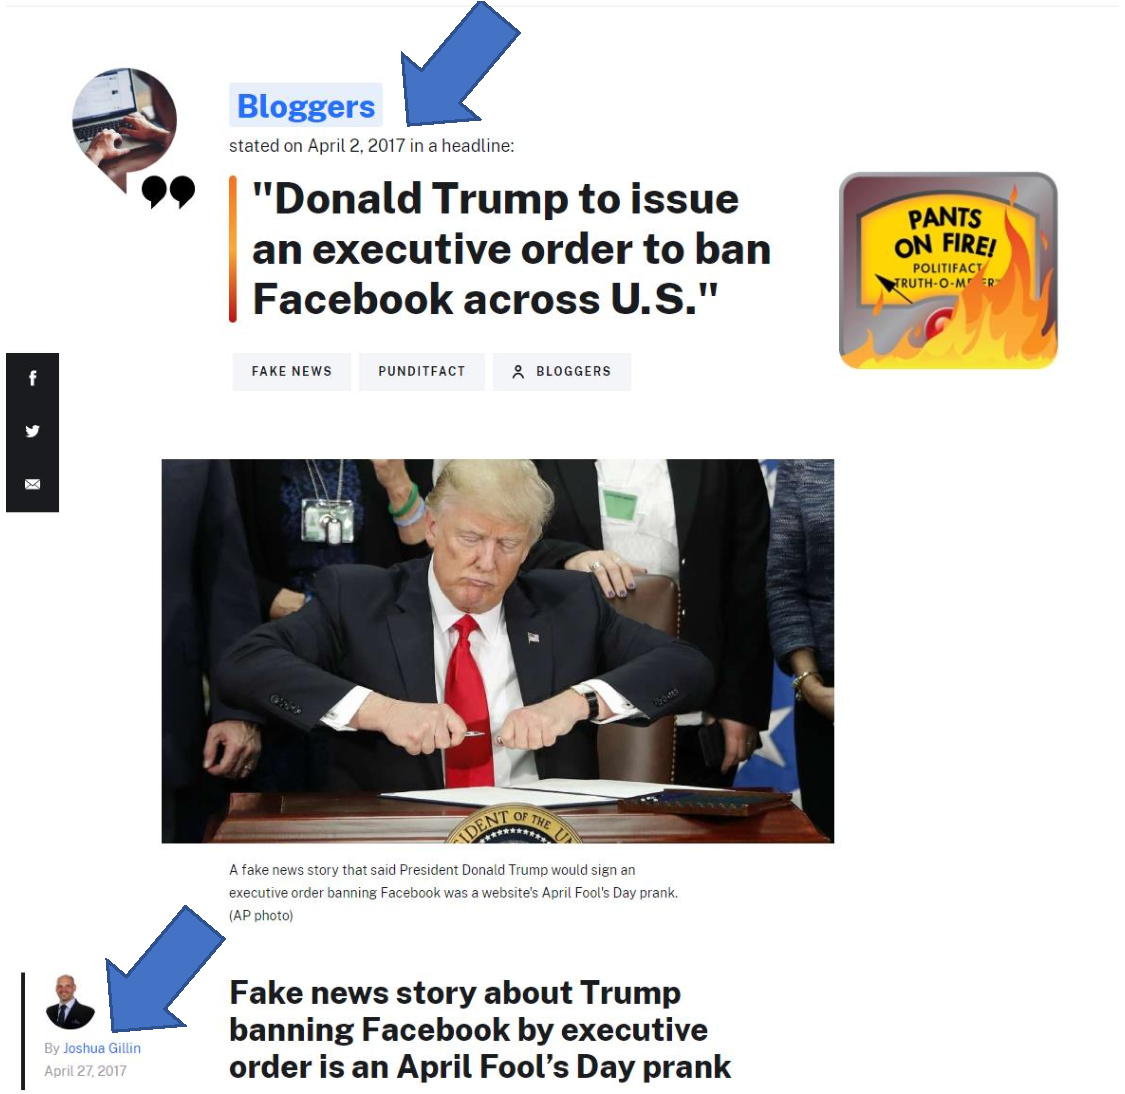
\includegraphics[width=0.7\linewidth]{images/fact-check.pdf}
  \caption{
      北米で行われたファクトチェックの一例。
      % この情報はエイプリルフールで投稿された虚偽情報としている。
      青矢印はフェイクニュース投稿日時とファクトチェック結果投稿日時を示し、両者には25日もの間が開いている。
      }
  \label{fig:example}
\end{figure}

\section{手法}

%先行研究により、自然言語文章生成モデルは言語モデルの1つとされており、式\ref{eq:generate}のように
%文章$x = \mathrm{w}_1^T = (\mathrm{w}_1, \mathrm{w}_2, ..., \mathrm{w}_T)$
%はある単語$\mathrm{w}_t$が生成される前の単語群$ \mathrm{w}_1^{t-1}$による条件付き確率の総積であると定義されている。

%\begin{equation}
%    \label{eq:generate}
%    p(x) = p(\mathrm{w}_1^T) = \prod_{t=1}^{T} p(\mathrm{w}_t|\mathrm{w}_1^{t-1})
%\end{equation}

提案モデルによる文章生成の流れは図\ref{fig:method}の通りである。
%\ref{subsec:generate}節の通り、Groverモデルでは記事を5要素に分けて学習が行われており、
%生成及び分類学習において、各要素の始点と終点には開始及び終了トークンが付加されている。
%本研究ではこれらの要素を記事本文とそれに寄せられた3件のコメントに置換することで実装する。
本研究ではベースとなったGroverモデル\cite{NIPS2019_9106}に倣い、提案モデルは以下の同時分布として定義する。

\begin{equation}
    \label{eq:joint_distri}
    p(\rm{article}, \rm{comment\_1}, \rm{comment\_2}, \rm{comment\_3})
\end{equation}

コメント生成学習時は、ベースとなったGroverモデルと同様に記事とコメントのセットを2つの集団に分け、無作為に要素を削除する。
コメントの場合は10\%、記事本文の場合は35\%の確率で歯抜けにしてから一方の集団から学習を行い、もう一方での生成におけるクロスエントロピー誤差を最小化するように訓練される\cite{NIPS2019_9106}。
%提案モデルの目的は記事ではなくSNS上で記事に寄せられたユーザの反応を生成することである。

\begin{figure}[t]
    \centering
    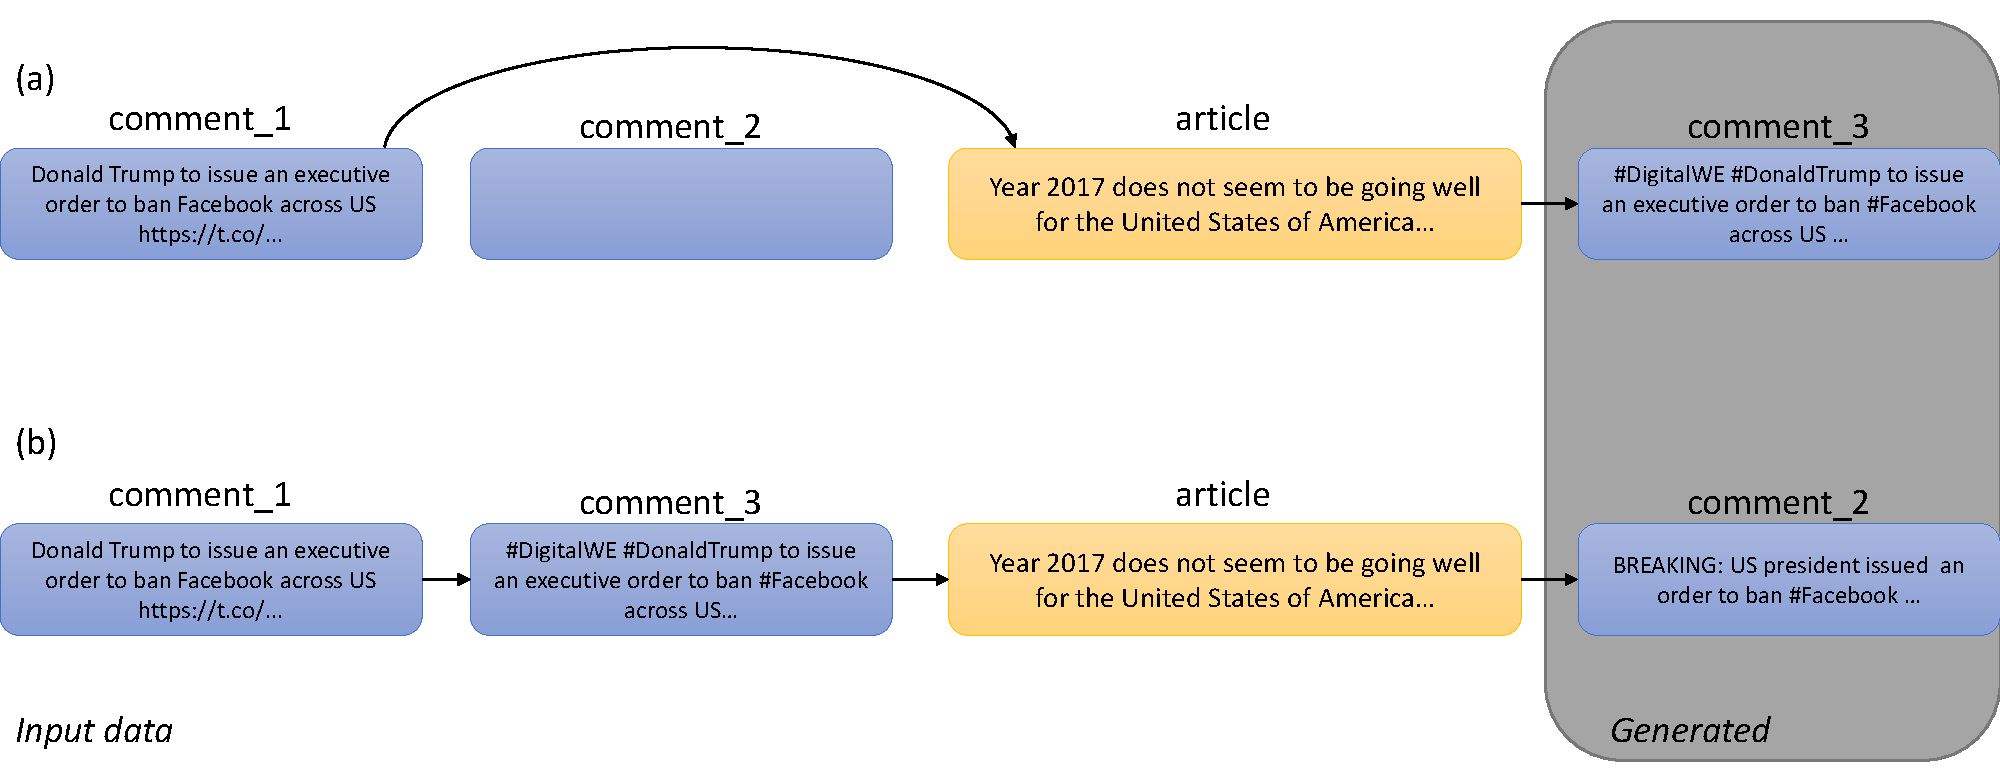
\includegraphics[width=\linewidth,pagebox=cropbox,clip]{images/fig_method.pdf}
    \caption{
        提案モデルのコメント生成例。
        (a)は記事と1件の実際に寄せられたコメントからコメントを生成している。
        (b)は(a)で生成したコメントを含めた状況で更にコメントを生成している。
    }
    \label{fig:method}
\end{figure}

記事とコメントのセットの末尾にはセットの終端を意味するトークンである\texttt{[CLS]}を追加し、またこのトークンが真偽を分類する際に使われる。
これはGroverモデルがベースとしているGPT-2がとる手法\cite{Radford_GPT2}と同一である。
図\label{fig:process}は実際の記事とコメントのセットを真偽分類するまでの流れである。
まず、記事に寄せられたコメント群から実験に使用するために無作為に3件選出し、コメント生成学習する。
真偽分類では、3件の実際に投稿されたコメントから1件削除し生成されたコメントを追加し真偽分類する。
%また、同時に生成コメントを追加しなかった状況で分類を行った際の結果との比較も行った。

\begin{figure}[t]
    \centering
    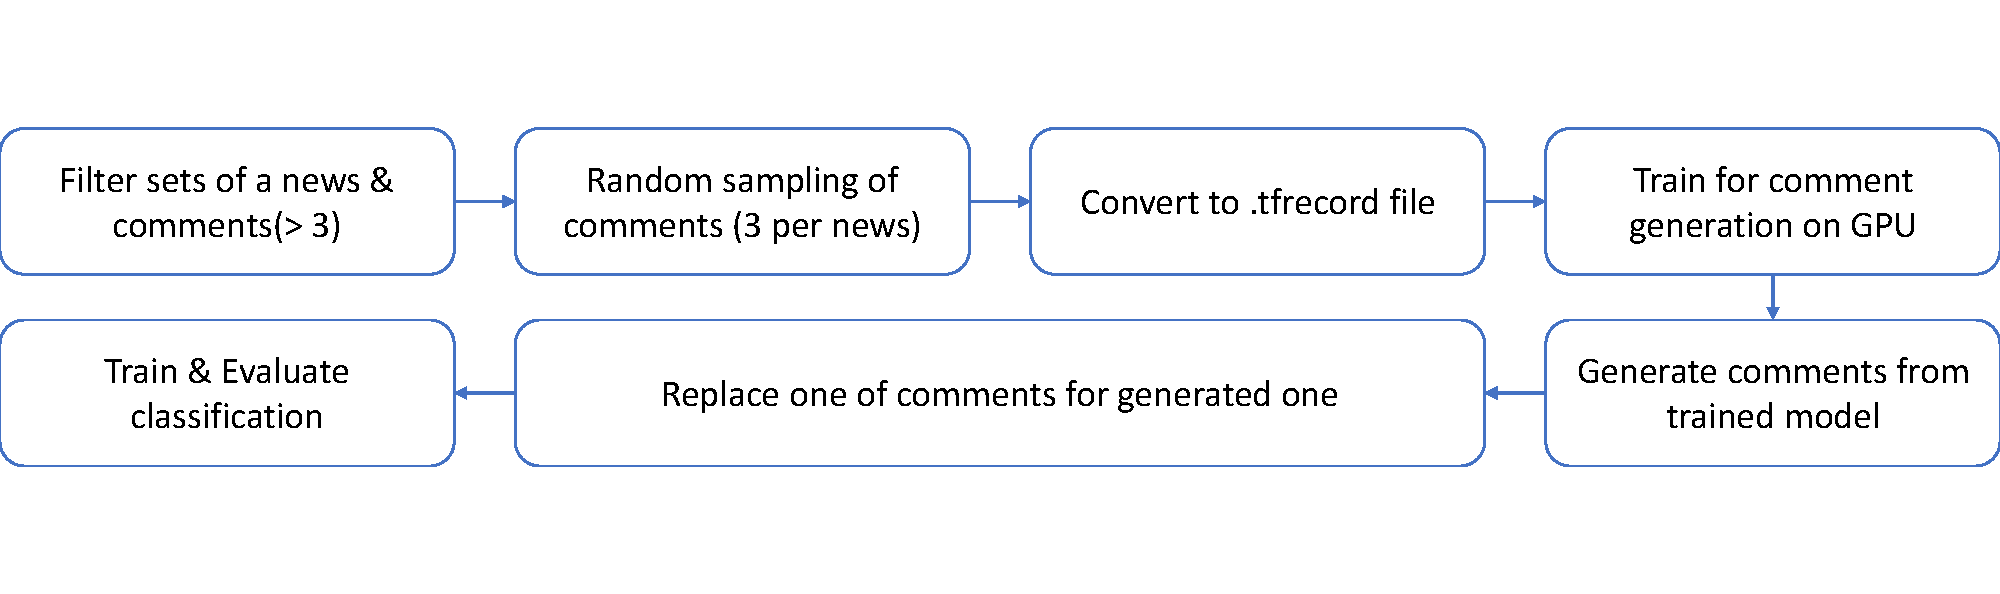
\includegraphics[width=\linewidth,pagebox=cropbox,clip]{images/fig_process.pdf}
    \caption{実験の流れ}
    \label{fig:process}
\end{figure}

\section{実験}

ニュース記事とコメントのセットはFakeNewsNetデータセット\cite{Shu2018FakeNewsNetAD}から取得した。
このデータセットは北米で英文記事を対象にファクトチェックを行う団体であるPolitiFact(政治ニュース中心)とGossipCop(芸能ニュース中心)の判断結果を元に正しいニュースとフェイクニュースのラベルが付けられている。
我々はまず実験手法に合わせるために記事に対して最低3件以上コメントが寄せられているセットに対して無作為に3件選出した。
生成コメントの有無によって真偽分類の結果に影響が出るか調べた。
ベースラインとして2つの入力データを用意した。
1つは生成されたコメントを入力せず、記事と実際に投稿された2件のコメントから分類させた場合、
もう1つは実際に投稿されたコメントも入力せず、記事のみから分類させた場合であった。
この実験では、PolitiFactでは十分な量の学習を行うにはセット数が少なかったため、GossipCopから真偽で各2000セットを用意して行った。

\section{結果}

実験結果は表\ref{tbl:classify_results}の通りである。
提案モデルは再現率において全体ベストとなったものの、適合率においては生成モデルを使わない方が優秀であることが読み取れる。
また、生成されたコメントには共通して文法面にさらなる改善の必要性が残された。

\begin{table}[!t]
  %\renewcommand{\arraystretch}{1.3}
  \caption{分類成績}
  \label{tbl:classify_results}
  \centering
  \begin{tabular}{lccc}
      \hline
      入力データ           & 適合率 & 再現率 & F値 \\ \hline\hline
      記事本文のみ         & 0.647     & 0.615  & 0.631    \\
      + 実在コメント2件  & \textbf{0.682}     & 0.750  & \textbf{0.714}    \\
      + 生成コメント1件 & 0.590     & \textbf{0.790}  & 0.675    \\ \hline
  \end{tabular}
\end{table}

\section{考察}
%\subsection{コメント生成}
%コメント生成の傾向から、提案モデルは入力されたニュース記事が扱うトピックの学習に成功したように見える。
%生成されたコメントの多くが政治的内容を含むものが多かった理由として、データセットが扱う内容の影響を受けたことが考えられる。

%生成コメントの中で興味深い単語は``breaking:''である。
%この単語はフェイクニュースに寄せられたコメントとして生成されていた。
%本研究と同じくコメントとして尤もらしい単語を生成するTCNN-URG\cite{ijcai2018-533}でも、
%フェイクを示すシグナルとして``!''や``?''、そして``false''が報告されていたが、``breaking:''は報告されていなかった。
%よって、この``breaking:''もフェイクニュースを示す重要なシグナルである可能性がある。

%生成されたコメントは文法面に改善点が残されているが、これはデータセットの規模不足が原因として考えられる。
%Groverモデルは120GBにも及ぶニュースデータセットから訓練されていた\cite{NIPS2019_9106}ことも考慮すると、
%改善のためにはさらなる追加データを収集する必要がある可能性が示されている。

%\subsection{真偽分類}
表\ref{tbl:classify_results}より、提案モデルは再現率は優秀だったが適合率に大きな課題を残した。
これはソーシャルコンテキストが制限されている状況でも、提案モデルにより多くのフェイクニュースの検出ができることを意味する。

この傾向はファクトチェックが必要なニュースを探す際に役立つことを示唆している。
ただし適合率が低く他のモデルより多く正しいニュースをフェイクニュースとして誤って検出するため、性能の改善が求められている。
今後は、より多くのデータセットを用いた場合に傾向が変化するか調べる必要がある。


\section{結論}
本研究では、フェイクニュースの早期発見における問題点の解決を試みた。
我々は、ユーザのコメントはニュース記事を評価する際で重要な情報をもたらすものの、
ニュース拡散の初期段階ではコメントが少ない点に着目する。
そこで、Groverモデルを拡張したニューラルネットワークモデルを作成し、分類に有用なコメントを生成することを提案する。
提案モデルのコメント生成による早期発見性能を評価するために、実際のニュースとそれに寄せられたコメントを対象に実験を行った。
その結果、コメントを生成するプロセスが、ファクトチェックによって真偽を判定する際に役立つ可能性が示唆されている。

{\small
\bibliographystyle{junsrt}
\bibliography{reference}
}
\end{document}
